%% This is an example first chapter.  You should put chapter/appendix that you
%% write into a separate file, and add a line \include{yourfilename} to
%% main.tex, where `yourfilename.tex' is the name of the chapter/appendix file.
%% You can process specific files by typing their names in at the 
%% \files=
%% prompt when you run the file main.tex through LaTeX.

\chapter{Case Studies}\label{Chap:CaseStudies}

This chapter presents the three case studies used to evaluate the webauthn firewall. Each case study involves using the webauthn firewall on a web service that is unique in some fundamental way. The variability stress tests the firewall's two main objectives: minimal intrusiveness and ease of configuraiton. The case studies provided valuable data on what aspects of the firewall need configuration and precisely what level of generalization is beneficial without becoming overly burdensome.

\section{Conduit}

Conduit is a simple RESTful blog web service \cite{TODO-conduit}. It is not a production product, rather an educational piece to demonstrate the flexibility of RESTful web-applications. The project supplies many simple frontend and backend implementations, done in various programming languages and frameworks, but following the same API specification. This way, they can be interchanged without problem. The case study focused on a React based frontend \cite{TODO-Conduit-React-Frontend} and a Golang based backend \cite{TODO-Conduit-Go-Backend}. Conduit is the best-case application for the webauthn firewall, a RESTful web service with basic functionality to protect. Absolutely no backend modifications are necessary to integrate webauthn.

%% \subsubsection{User Identification}
%% TODO: Maybe talk about JWT

\subsection{Context Retrieval}\label{Sec:Conduit_ContextRetrieval}

A major benefit of a RESTful web-application is that the backend intentionally exposes many useful context routes. By design, a RESTful frontend performs the necessary rendering on the user's web-browser, but must retrieve user specific information from the backend. This is essentially equivalent to webauthn context retrieval discussed in Section~\ref{Sec:ContextRetrieval}. For example, the backend already implements routes such as getting an article by its ID. And if not, then there certainly will be a tangential route such as requesting all comments of an article to search for a specific one by ID. Since most of the modifications necessary to the backend when integrating the webauthn firewall are for context routes, this aspect of RESTful applications make that easy.

\subsection{Secured Routes}

The simplicity of the Conduit application did not challenge the domain specific language much. The domain specific programs simply retrieve some context to complete the format strings. However, the user settings route does require a custom handler since transaction authentication. It too is not exceptionally complicated, where the route is only protected if the username, email or password are modified. Otherwise, HTTP requests to modify only the bio or profile pictures pass through without any verification.

\section{Calypso}

Calypso is a RESTful frontend for a WordPress admin panel \cite{TODO-calypso}. This is a production product, with far greater complexity than the Conduit application. Also, unlike Conduit with a backend running locally which may be modified, Calypso accesses the official WordPress backend servers. These servers are closed-source and their modification is out of question. Whereas avoiding backend modifications for Conduit is a favorable result, with Calypso it is a necessity. Nonetheless, integrating webauthn is possible because the RESTful API of WordPress was complete enough to satisfy the needs of the webauthn firewall.

\subsection{Multi-Target Proxying}

\begin{figure}[h]
  \centering
  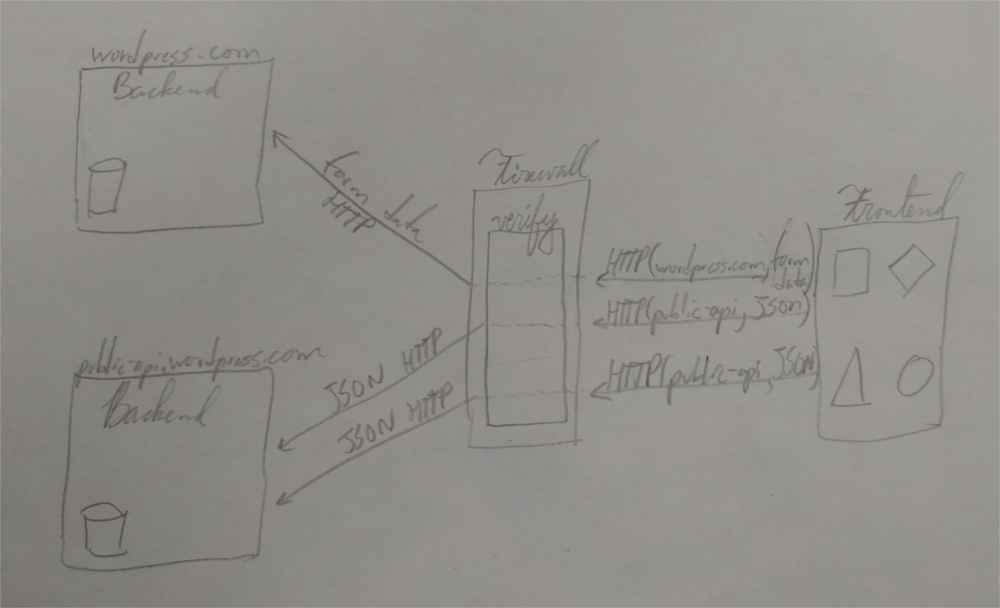
\includegraphics[width=12cm]{multitarget_calypso}
\end{figure}

Unlike the other two case studies, a point of complexity that Calypso has is that the frontend accesses multiple backends. Typically, the frontend requests to a single backend source. WordPress has a backend for API requests, \lstinline{"public-api.wordpress.com"}, that accepts JSON payloads. Most of Calypso interacts with this backend. However, login requests go to the regular \lstinline{"wordpress.com"} backend which uses form-data payloads. This prompts the firewall to support multi-target proxying. Requests sent to the firewall contain their destined targets in their headers, and the firewall proxies accordingly. The firewall configuration for Calypso lists both of those target domains along with \lstinline{GetJSONInput} and \lstinline{GetFormInput} as their default input handlers respectively. 

\subsection{Login}\label{Sec:CalypsoLogin}

The webauthn firewall automatically protects a number of core webauthn routes, including the route for login, as described in Section~\ref{Sec:DefaultHandlers}. However, the Calypso project approaches login in an atypical fashion. Normally a service has a dedicated route for login. Calypso shares a login route with other operations, so HTTP requests are identified by an \lstinline{"action"} field in their payload, similarly as described in~\ref{Sec:CustomHandlers}. As a result, the default login handler could not support Calypso out of the box. Extending the default login handler to be customizable for this one specific case would make the firewall's configuration too complicated. Rather, a custom login handler implements the Calypso login event. The login handler roughly resembles the following Go pseudo-code.

\begin{lstlisting}[float=h]
func finishLogin(w http.ResponseWriter, req *wf.ExtendedRequest) {
  action := req.Get("action")
  switch action {
    case "login-endpoint":
      // Webauthn verify the login request
      VerifyLogin(w, req)
    default:
      // Other requests go right through
      ProxyRequest(w, req)
  }
}
\end{lstlisting}

\subsection{Secured Routes}\label{Sec:CalypsoSecuredRoutes}

The power of the domain specific language begins to shine with Calypso. Certain domain specific programs have multiple context retrievals. Others have multiple format tags to fill, and one program requires a special formatting function. Apart from the custom login handler, all of the routes in Calypso are protected using the DSL. There is no case where a custom handler is necessary. One route receives HTTP request containing an array of elements that need to be comma separated in the authentication message. Rather than implementing a custom handler for this minor inconvenience, the \lstinline{Apply} domain specific operation described in Table~\ref{Table:DSL_GetterOperations} resolves this problem. Essentially, it enables Go code to be used within a domain specific program to a limited extent. The following is a domain specific program for inviting new users to administer a WordPress blog.

\begin{lstlisting}[float=h]
firewall.Secure("POST", "/rest/{version}/sites/{site_id}/invites/new", 
  firewall.Authn("Invite new user(s): %v",
  wf.Apply(func(args ...interface{}) (interface{}, error) {
    invitees := args[0].([]string)
    return strings.Join(invitees, ","), nil
  }, wf.GetArray("invitees")),
))
\end{lstlisting}

The \lstinline{Authn} operation string formats the argument of \lstinline{wf.GetArray("invitees"))} with the full power of the Go programming language.

\section{Gogs}

Gogs is a server-side rendered self-hosted Git web service \cite{TODO-gogs}. A server-side rendered web-application presents its own set of challenges to the webauthn firewall. Section~\ref{Sec:ProxyingRequests} explains how the firewall has to be the end-point interacting with the user's web-browser. Apart from that, context must be served by the Gogs backend. It does not have the convenience of automatically exposing context routes like RESTful backends as discussed in Section~\ref{Sec:Conduit_ContextRetrieval}.

\subsection{Intrusive Webauthn}

The Gogs web service was the first case-study of the three studied. Before the webauthn firewall became a mature idea, part of Gogs was secured in the traditional, intrusive fashion presented in Section~\ref{Sec:StatusQuo}. The intrusive approach was abandoned once the firewall proved itself a prospective mechanism and all of the work redone. The two main challenges with integrating webauthn into Gogs intrusively are the database adapter and organizational difficulties. Webauthn needs a database table to record entries of users' public key credentials. Simply creating a new table in Gogs requires writing a custom database adapter for that table and modifying the codebase in a number of disjoint locations. Furthermore, the handlers for various Gogs routes are interspersed all around the code. Keeping track of which routes are webauthn secured becomes increasingly more difficult as more routes are protected.

\subsection{Context Retrieval}

A downside to server-side rendering web services when compared to RESTful services when it comes to webauthn firewall integration is the lack of pre-built context routes. Effectively, the API routes in the RESTful backend services act as the context routes. Gogs, being a server-side rendering backend, needs to be modified to include those context routes. Some Gogs routes need additional context to retrieve objects such as a \lstinline{"repository"} or \lstinline{"webhook"}. Gogs serves this context information out of a \lstinline{"server_context/<type>/<args>"} route. The \lstinline{<type>} refers to what type of object is being requested, i.e. repository, webhook, etc. Each context type gets its own handler in Gogs which interprets the \lstinline{<args>} to retrieve the correct context object.

%% 
%% \iffalse
%% As the Gogs routes get webauthn protected, becomes more evident which 
%% \fi
%% 

\subsection{Custom Handlers}

As with the other case-studies, most of the routes are simple and easy to secure using the domain specific language. At most, they require a singular context retrieval to fill a single format tag. Within the Gogs service, there are a number of routes that are shared by multiple HTTP operations. Similarly to the login route of Calypso discussed in Section~\ref{Sec:CalypsoLogin}, there is an \lstinline{"action"} field in the HTTP request payload which delineates the operation type. Only certain actions warrant being transaction authenticated. Custom handlers are used in these cases, to parse the \lstinline{"action"} field and webauthn secure only when necessary.

Gogs requires a more involved custom handler for protecting publishing a new releases. The files associated with a new release are contained as UUIDs in the HTTP request. So each file needs context retrieval to get the file name which then correctly must be comma separated in the format string. Rather than expressing this series of operations and formatting in an \lstinline{Apply} operation like with Calypso in Section~\ref{Sec:CalypsoSecuredRoutes}, it is best to drop down to a custom handler function. The following code snippet is Go pseudo-code for the custom handler.

\begin{lstlisting}[float=h]
func publishNewRelease(w http.ResponseWriter, r *wf.ExtendedRequest) {
  title := r.Get("title")
  uuids := r.Request.Form["files"]

  names := []string{}
  for _, uuid := range uuids {
    append(names, r.GetContext("attachment", uuid)["Name"].(string))
  }

  authText := fmt.Sprintf("Publish release named: %v", title)
  authText += fmt.Sprintf("\nFile names: %s", strings.Join(names, ", "))

  handlerFn := firewall.Authn(authText)
  handlerFn(w, r)
}
\end{lstlisting}

%% 
%% \iffalse
%% Essentially, the firewall assumes the roles of the frontend in the RESTful use-cases. 
%% \fi
%% 
